\documentclass[main.tex]{subfiles}
\begin{document}

\subsection{Show that the 10 matrices $\frac{1}{2}\sigma_a\otimes\mathbb{I}$, $\frac{1}{2}\sigma_a\otimes\tau_1$, $\frac{1}{2}\sigma_a\otimes\tau_3$, $\frac{1}{2}\mathbb{I}\otimes\tau_2$ generate the spinor representation of $\mathfrak{so}(5)$. Find the matrix $R=R^{-1}\st T_a=-RT_a^*R$.}

Take the Cartan subalgebra to be
\begin{equation}
H_1=\frac{1}{2}\sigma_3\otimes\mathbb{I}=\frac{1}{2}\begin{pmatrix}1&0&0&0\\
0&1&0&0\\0&0&-1&0\\0&0&0&-1\end{pmatrix},\quad H_2=\frac{1}{2}\sigma_3\otimes\tau_3=\frac{1}{2}\begin{pmatrix}1&0&0&0\\
0&-1&0&0\\0&0&-1&0\\0&0&0&1\end{pmatrix}
\end{equation}  
which have eigenvalues $\lambda=\pm\frac{1}{2}$. The eigenvectors and associated weights are
\begin{align}
x_1=\begin{pmatrix}1\\0\\0\\0\end{pmatrix}&\quad \mu_1=(\frac{1}{2},\frac{1}{2})\\
x_2=\begin{pmatrix}0\\1\\0\\0\end{pmatrix}&\quad \mu_2=(\frac{1}{2},-\frac{1}{2})\\
x_3=\begin{pmatrix}0\\0\\1\\0\end{pmatrix}&\quad \mu_3=(-\frac{1}{2},-\frac{1}{2})=-\mu_1\\
x_4=\begin{pmatrix}0\\0\\0\\1\end{pmatrix}&\quad \mu_4=(-\frac{1}{2},\frac{1}{2})=-\mu_2.
\end{align}

The spinor rep of $\mathfrak{so}(5)$ is $\left|\pm \frac{e^1}{2}\pm \frac{e^2}{2}\right>$ with $e^1=(1,1)=-(-1,-1)$, $e^2=(1,-1)=-(-1,1)$. Thus the matrices generate the spinor rep of $\mathfrak{so}(5)$ with $\pm\mu_1=\pm\frac{1}{2}e^1$, $\pm\mu_2=\pm\frac{1}{2}e^2$.

Then to find the matrix $R$, when we know that from the Hermitian generators $\sigma_3\otimes\tau_2$, $\sigma_3\otimes\tau_1$ we can construct all of the other generators via commutation, thus we may find the $R$ for which $T_a=-RT_a^*R^{-1}$. Let $R=r^1\otimes r^2$. So, using $\sigma_3^*=\sigma_3$, $\sigma_1=\sigma_1$ \& $\sigma_2^*=-\sigma_2$.
\begin{align}
\sigma_3\otimes\tau_2=&-r^1\sigma_3^*{r^1}^{-1}\otimes r^2\tau_2^*{r^2}^{-1}\\
=&r^1\sigma_3{r^1}^{-1}\otimes r^2\tau_2{r^2}^{-1}
\end{align}
and
\begin{align}
\sigma_3\otimes\tau_1=&-r^1\sigma_3^*{r^1}^{-1}\otimes r^2\tau_1^*{r^2}^{-1}\\
=&-r^1\sigma_3{r^1}^{-1}\otimes r^2\tau_1{r^2}^{-1}.
\end{align}
Pick $r^1=\sigma_2$ and $r^2=\tau_1$ which gives the desired properties, so $R=\sigma_2\otimes\tau_1$.

\subsection{Determine how the spinor rep of $\mathfrak{so}(2n+1)$ transforms under the $\mathfrak{so}(2n-1)$ subalgebra.}
$\mathfrak{so}(2n-1)$ can be generated by the products of of $n-1$ Pauli matrices $\sigma_a^1\otimes\sigma_a^2\otimes...\otimes\sigma_a^{n-1}$ with the raising/lowering ops given by $E_{\pm e^j}=\frac{1}{2}\sigma_3^1\otimes...\otimes\sigma_3^{j-1}\otimes\sigma_1^j\otimes...\otimes\mathbb{I}^{n-1}$.
Acting with the $\mathfrak{so}(2n-1)$ operators on the full $\mathfrak{so}(2n+1)$ spinor rep $\left|\pm\frac{e^1}{2}\pm\frac{e^2}{2}...\pm\frac{e^n}{2}\right>$ produces the same transformation on the first $\pm e^1/2...\pm e^{n-1/2}$ terms as under the full $\mathfrak{so}(2n+1)$ operators, but the $\pm e^n/2$ state is invariant under $\mathfrak{so}(2n-1)$ thus the spinor rep of $\mathfrak{so}(2n+1)$ is not an irrep under the $\mathfrak{so}(2n-1)$ sub-algebra. This can be seen from the Dynkin diagram 

\begin{center}
  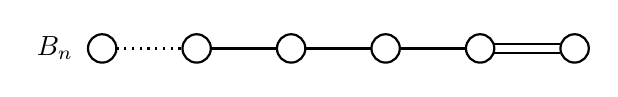
\begin{tikzpicture}[scale=.6]
    \foreach \x in {0,...,4}
    \draw[xshift=\x cm,thick] (\x cm,0) circle (.3cm);
    \draw[xshift=5 cm,thick] (5 cm, 0) circle (.3 cm);
    \draw[dotted,thick] (0.3 cm,0) -- +(1.4 cm,0);
    \foreach \y in {1.15,...,3.15}
    \draw[xshift=\y cm,thick] (\y cm,0) -- +(1.4 cm,0);
    \draw[thick] (8.3 cm, .1 cm) -- +(1.4 cm,0);
    \draw[thick] (8.3 cm, -.1 cm) -- +(1.4 cm,0);
    \node at (-1,0) {$B_n$};
  \end{tikzpicture}
\end{center}

has a 
\begin{center}
  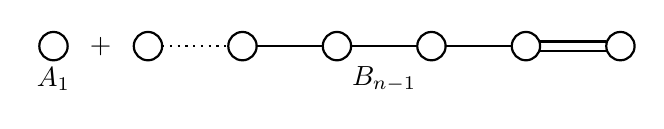
\begin{tikzpicture}[scale=.6]
    \draw[thick] (-2,0) circle (.3cm);
    \node at (-1,0) {$+$};
    \foreach \x in {0,...,4}
    \draw[xshift=\x cm,thick] (\x cm,0) circle (.3cm);
    \draw[xshift=5 cm,thick] (5 cm, 0) circle (.3 cm);
    \draw[dotted,thick] (0.3 cm,0) -- +(1.4 cm,0);
    \foreach \y in {1.15,...,3.15}
    \draw[xshift=\y cm,thick] (\y cm,0) -- +(1.4 cm,0);
    \draw[thick] (8.3 cm, .1 cm) -- +(1.4 cm,0);
    \draw[thick] (8.3 cm, -.1 cm) -- +(1.4 cm,0);
    \node at (5,-0.7) {$B_{n-1}$};
    \node at (-2,-0.7) {$A_{1}$};
  \end{tikzpicture}
\end{center}
$=\mathfrak{su}(2)+\mathfrak{so}(2n-1)$ subalgebra. 
\end{document}